%%%%%%%%%%%%%%%%%%%%%%%%%%%%%%%%%%%%%%%%%
% Stylish Article
% LaTeX Template
% Version 2.1 (1/10/15)
%
% This template has been downloaded from:
% http://www.LaTeXTemplates.com
%
% Original author:
% Mathias Legrand (legrand.mathias@gmail.com) 
% With extensive modifications by:
% Vel (vel@latextemplates.com)
% Final ACS by:
% Juan Barbosa
% License:
% CC BY-NC-SA 3.0 (http://creativecommons.org/licenses/by-nc-sa/3.0/)
%
%%%%%%%%%%%%%%%%%%%%%%%%%%%%%%%%%%%%%%%%%
\documentclass[fleqn,11pt]{SelfArx}
%\usepackage[superscript]{cite}
\usepackage{wrapfig}
\usepackage{rotating}
\usepackage{subcaption}
\usepackage[numbers, super]{natbib}
%----------------------------------------------------------------------------------------
%	ARTICLE INFORMATION
%----------------------------------------------------------------------------------------

\JournalInfo{Laboratorio Org\'anica 3, No. 2, 15/09/2017} % Journal information
\Archive{ }

\PaperTitle{Reacci\'on de McMurry} %
%\Keywords{Keyword1 --- Keyword2 --- Keyword3} % Keywords - if you don't want any simply remove all the text between the curly brackets
%\newcommand{\keywordname}{Keywords} % Defines the keywords heading name

%----------------------------------------------------------------------------------------
%	ABSTRACT
%----------------------------------------------------------------------------------------

\Abstract{
\begin{wrapfigure}{r}{0.5\textwidth}
	\centering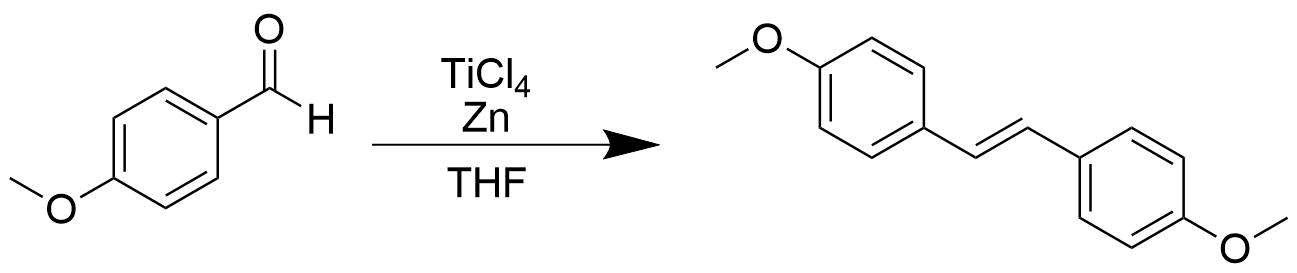
\includegraphics[width=\linewidth]{structures/Reaction.png}
\end{wrapfigure}

La preparaci\'on del (\textit{E})-1,2-bis(4-metoxifenil)eteno se llev\'o a cabo usando 4-metoxibenzaldehido, cloruro de titanio (IV) y zinc como agente reductor, en una reacci\'on de McMurry, usando tetrahidrofurano como disolvente. La reacci\'on tuvo una duraci\'on de 19 horas y un rendimiento de \_\_\_ \%. La caracterizaci\'on del producto se llev\'o a cabo usando $^1$HRMN y $^{13}$CRMN. 
}

%----------------------------------------------------------------------------------------

\begin{document}

\flushbottom % Makes all text pages the same height

\maketitle % Print the title and abstract box

%\tableofcontents % Print the contents section

\thispagestyle{empty} % Removes page numbering from the first page

%----------------------------------------------------------------------------------------
%	ARTICLE CONTENTS
%----------------------------------------------------------------------------------------

\section*{Introducci\'on} % The \section*{} command stops section numbering
%------------------------------------------------

La reacci\'on de McMurry fue publicada en 1974, por John E. McMurry. Si bien var\'ios art\'iculos fueron publicados en la d\'ecada de los 70 \cite{Mukaiyama1973, Mukaiyama1974} sobre reacciones de acoplamiento reductivo de carbonilos a alquenos usando esp\'ecies de titanio con bajo estado de oxidaci\'on, fue McMurry el que hizo un estudio detallado de los alcances de la reacci\'on \cite{Wang2010}.

Los alquenos producidos por este m\'etodo suelen ser mayoritariamente \textit{trans}, sin embargo existen casos donde se da el \textit{cis}. El control de la estereoqu\'imica en la reacci\'on de McMurry es limitado por el tama\~no de las mol\'eculas reactantes. Por otro lado la reacci\'on \'unicamente funciona con eficacia en los casos donde el acoplamiento se da entre compuestos arom\'aticos \cite{Wang2010}, sin embargo tambi\'en ocurre con menor frecuencia en compuestos alif\'aticos. Para que la reacci\'on se lleve acabo son necesarias altas temperaturas y tiempos prolongados para la desoxigenaci\'on de la mol\'ecula \cite{Wang2010, Villiers1997}.

\begin{scheme}[h]
	\centering
	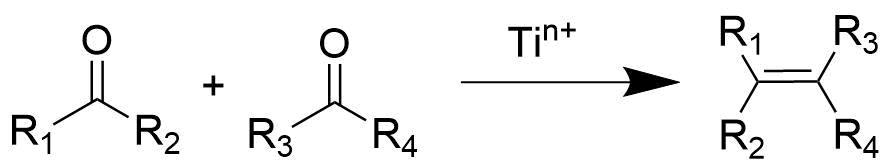
\includegraphics[width=0.9\linewidth]{structures/generalreaction.png}
	\caption{Reacci\'on general de McMurry. El estado de oxidaci\'on del titanio es $0<n<3$. \ce{R1, R3}: alquil o aril, \ce{R2, R4}: H, alquil o aril. \cite{Wang2010}}
\end{scheme}

La reacci\'on de McMurry es muy usada para la formaci\'on de alquenos a partir de aldeh\'idos, siendo una ventaja importante la posibilidad de realizar acoplamientos intra e intermoleculares de aldeh\'idos y cetonas en macrociclos \cite{Wang2010, Villiers1997}. La reacci\'on tiene lugar con titanio neutro, el cual se produce a partir de esp\'ecies de titanio con estados de oxidaci\'on $+2$, $+3$ y $+4$ producidos \textit{in situ}, con un agente reductor. Una gran cantidad de agentes reductores han sido usados en la reacci\'on de McMurry, ejemplos de estos son: \ce{Mg}, \ce{Zn}, \ce{LiAlH4}, \ce{LiBH4}, \ce{LiH}, \ce{CaH2} \cite{Wang2010}.

\begin{figure*}[ht]
	\centering
	\begin{subfigure}[t]{0.49\linewidth}
		\centering
		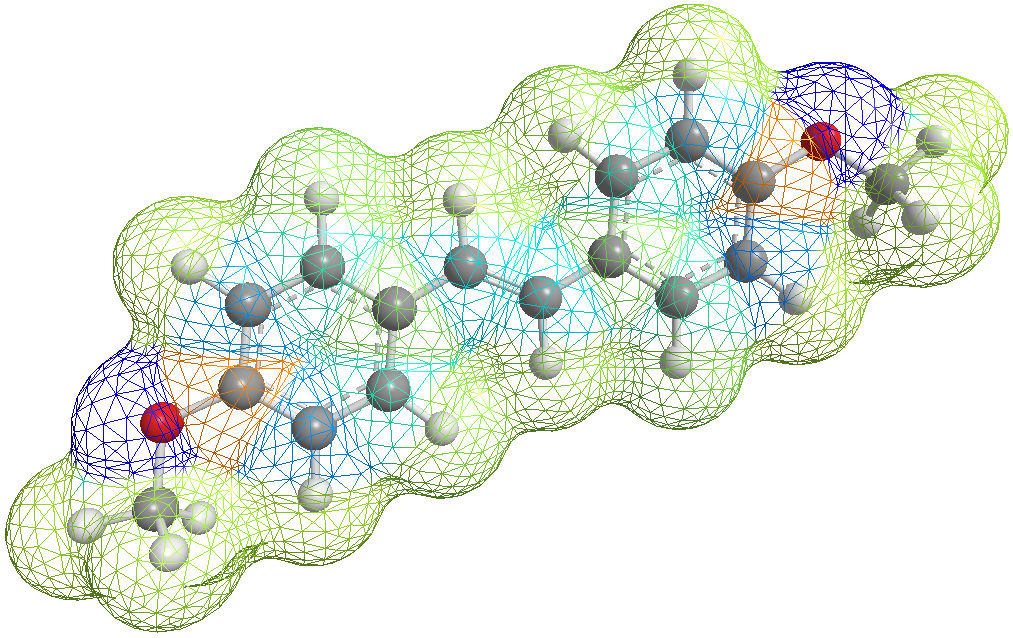
\includegraphics[width=0.9\linewidth]{structures/productE.png}
		\caption{(\textit{E})-1,2-bis(4-metoxifenil)eteno, $E=12.1013$ kcal/mol.}
	\end{subfigure}
	\begin{subfigure}[t]{0.49\linewidth}
		\centering
		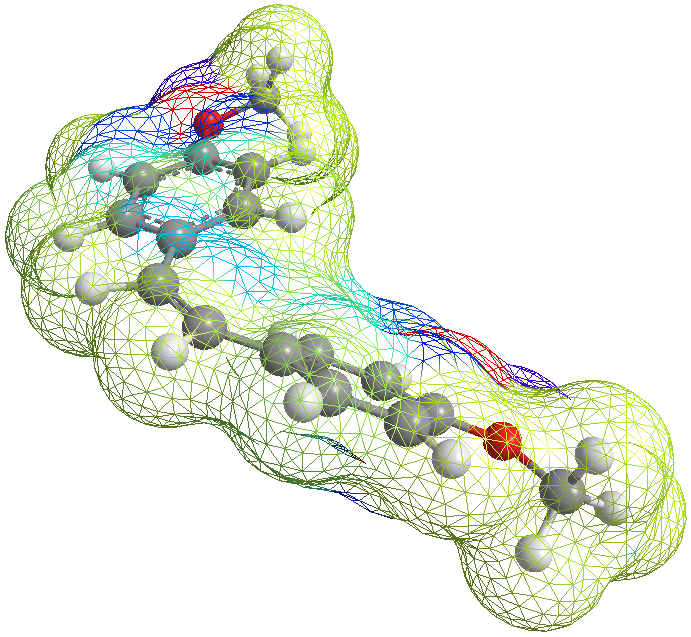
\includegraphics[width=0.7\linewidth]{structures/productZ.png}
		\caption{(\textit{Z})-1,2-bis(4-metoxifenil)eteno, $E=23.4982$ kcal/mol.}
	\end{subfigure}
	\caption{Estereoqu\'imica de los posibles productos de la reacci\'on de McMurry. El color viene de la densidad de carga: azul para los valores m\'inimos y rojo para valores m\'aximos.}
	\label{fig: both}
\end{figure*}

\newpage

\section{Resultados y Discusi\'on}
El titanio (IV) se reduce en presencia de zinc (\autoref{eq: reduccion}), la reacci\'on se lleva a cabo en tetrahidrofurano por dos razones: la primera es que el cloruro de titanio (IV) es soluble en THF, y por otro lado este disolvente no se reduce por las condiciones de la reacci\'on \cite{richards2001}. Esta etapa comprende la primera parte de la reacci\'on, la cual se lleva a cabo a reflujo por una hora.
\begin{equation}\label{eq: reduccion}
	\ce{TiCl4 + Zn ->[\Delta] TiCl2 + ZnCl2}
\end{equation}

El cloruro de titanio (II) formado \textit{in situ} puede a su vez reducirse nuevamente para formar el titanio met\'alico.
\begin{equation}
	\ce{TiCl2 + Zn ->[\Delta] Ti + ZnCl2}
\end{equation}

La segunda parte de la reacci\'on mecan\'isticamente se divide en dos etapas. La primera es la formaci\'on del pinacol seguida de la desoxigenaci\'on del mismo. Aquí se discuten dos posibles mecanismos para la reacci\'on de acoplamiento. En el \autoref{sch: primer} se muestra el primer mecanismo propuesto, una vez se adiciona el \textit{p}-metoxibenzaldehido al medio de reacci\'on un electr\'on de valencia del titanio ataca al ox\'igeno generando a su vez un radical sobre el carbono carbon\'ilico \textbf{(a)}. Posteriormente el radical de titanio ataca de forma an\'aloga a otra mol\'ecula de aldeh\'ido \textbf{(b)}. Luego tiene lugar la ciclaci\'on \textbf{(c)}, en este punto dos posibles intermediarios se pueden formar dependiendo de la orientaci\'on de los ciclos.
\begin{scheme}[h]
	\centering
	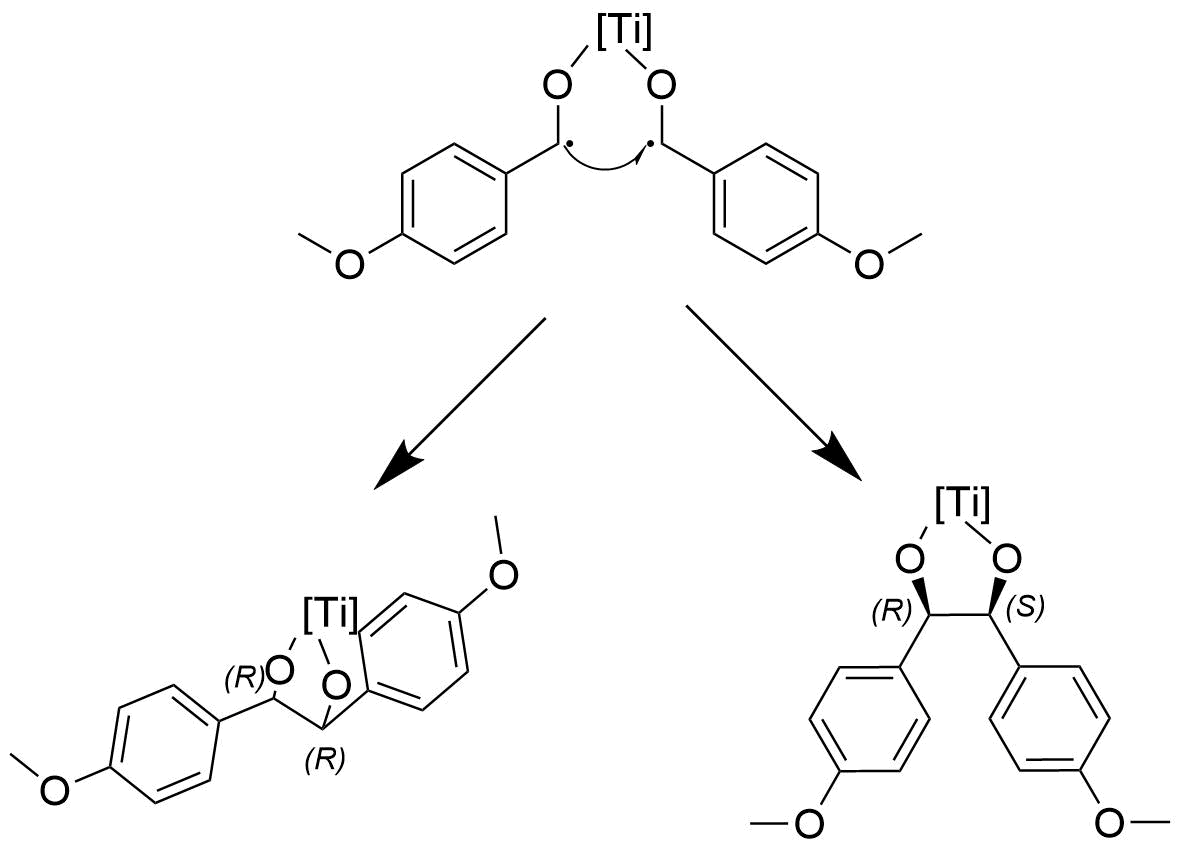
\includegraphics[width = 0.8\linewidth]{structures/EZdetermined.png}
	\caption{Posibles formas en las que tiene lugar la ciclaci\'on.}
	\label{sch: EZ}
\end{scheme}

\pagebreak

Teniendo en cuenta el volumen de los ciclos y las interacciones desfavorables que se tienen si ambos se encuentran muy cerca, la ciclaci\'on se da a manera de puente (\textit{R, R}), esto porque la energ\'ia total de la mol\'ecula con estereoqu\'imica (\textit{R, R}) es cerca de la mitad de la de estereoqu\'imica (\textit{R, S}) (\autoref{fig: both}). La informaci\'on de la energ\'ia es particularmente útil teniendo en cuenta que los estados de transici\'on y los productos de menor energ\'ia est\'an favorecidos. La formaci\'on de un pinacol \textbf{(d)}, da paso a la desoxigenaci\'on de la mol\'ecula, con la liberaci\'on del \'oxido de titanio (IV), generando el producto de estereoqu\'imica \textit{E} \cite{richards2001}. Cabe mencionar que seg\'un este mecanismo, si el ciclo formado en el paso \textbf{(c)} tiene la estereoqu\'imica (\textit{R, S}) el producto final ser\'a el \textit{Z} (energ\'eticamente desfavorable).
\begin{scheme}[h]
	\centering
	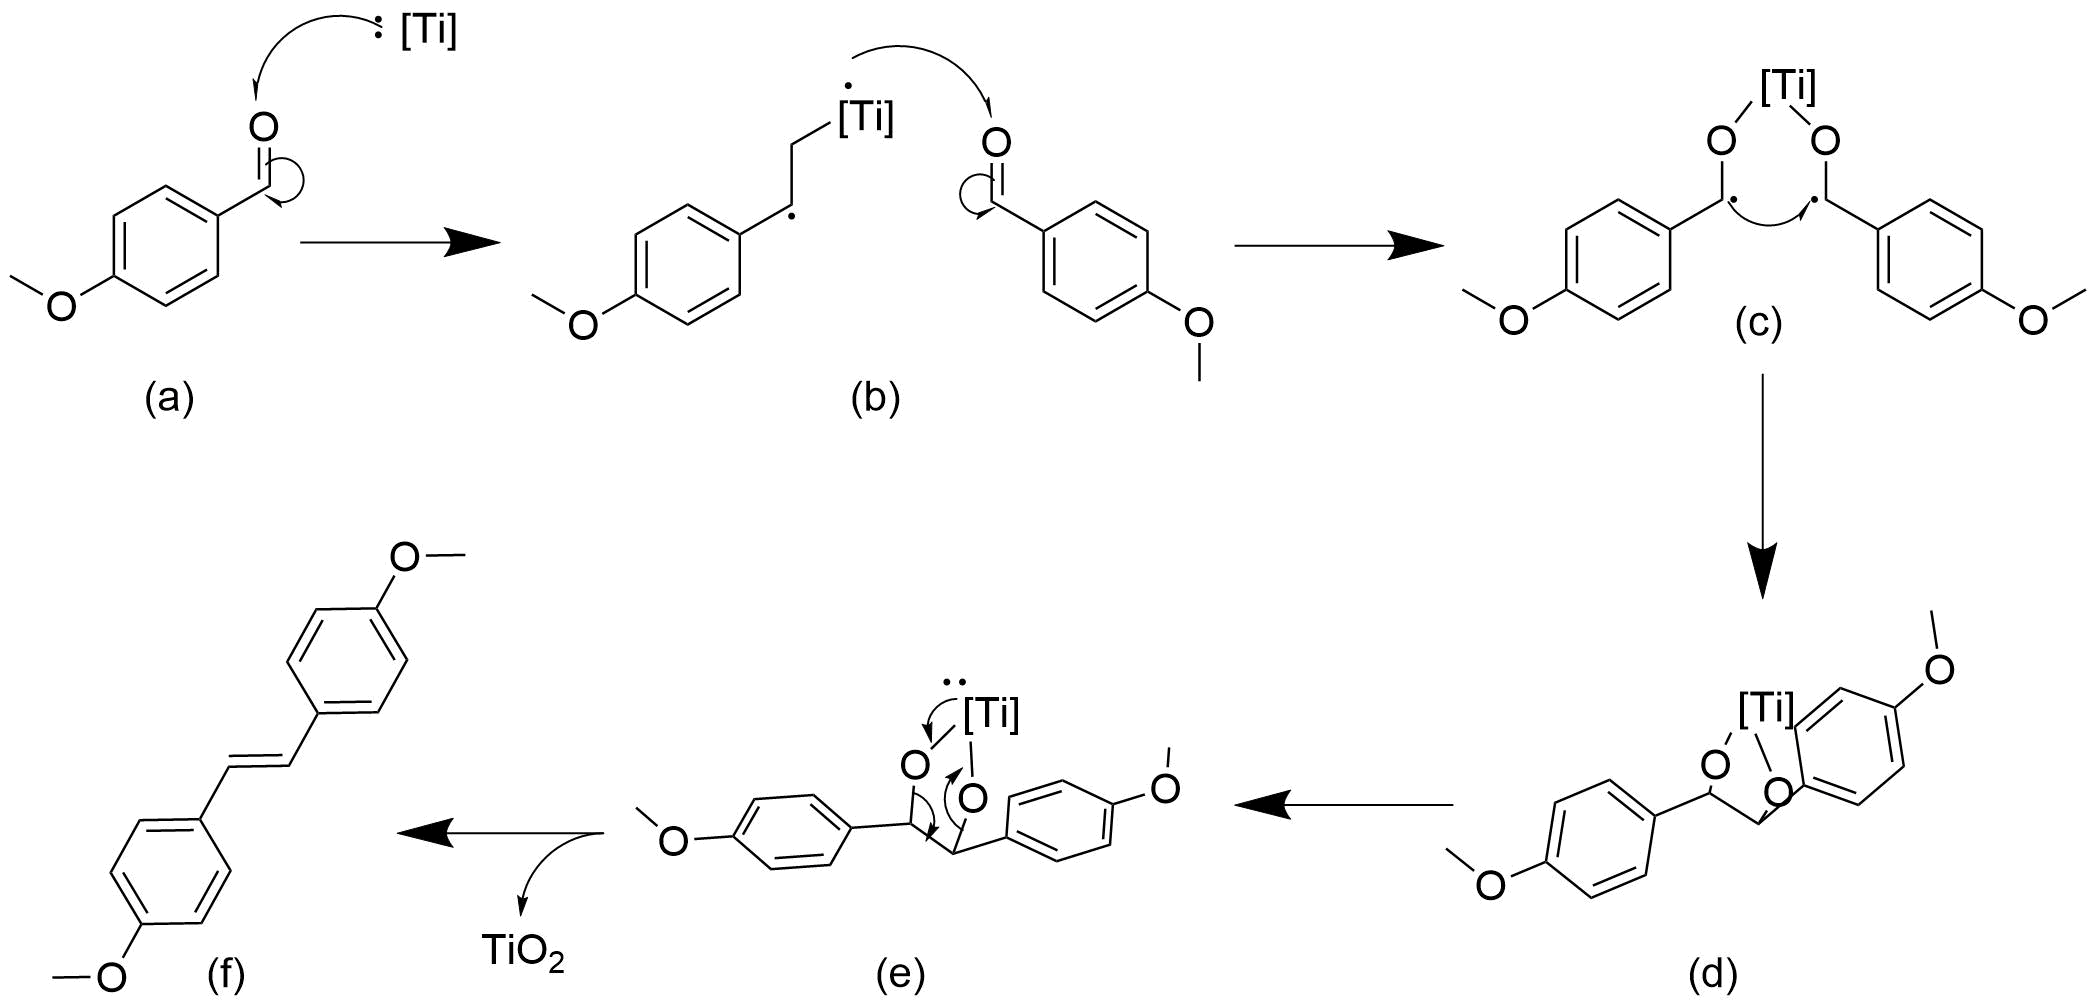
\includegraphics[width = \linewidth]{structures/mechanism.png}
	\caption{Primer mecanismo de reacci\'on propuesto.}
	\label{sch: primer}
\end{scheme}

El segundo mecanismo propuesto involucra una relaci\'on estequeom\'etrica titanio-producto (4:1). En este caso el ataque del titanio se da por aparte en dos mol\'eculas de \textit{p}-benzaldeh\'ido \textbf{(g)}. Posteriormente tiene lugar el acoplamiento con los radicales, en este paso tambi\'en es posible que se formen los estereois\'omeros (\textit{R, R}) \'o (\textit{R, S}) an\'alogo al \autoref{sch: EZ}. Posteriormente tiene lugar la desoxigenaci\'on con la formaci\'on de un nuevo enlace titanio \'oxigeno sobre los dos ox\'igenos de la mol\'ecula, y la formaci\'on de un enlace $\pi$ carbono-carbono \textbf{(j)} \cite{Wang2010}.
\begin{scheme}[h]
	\centering
	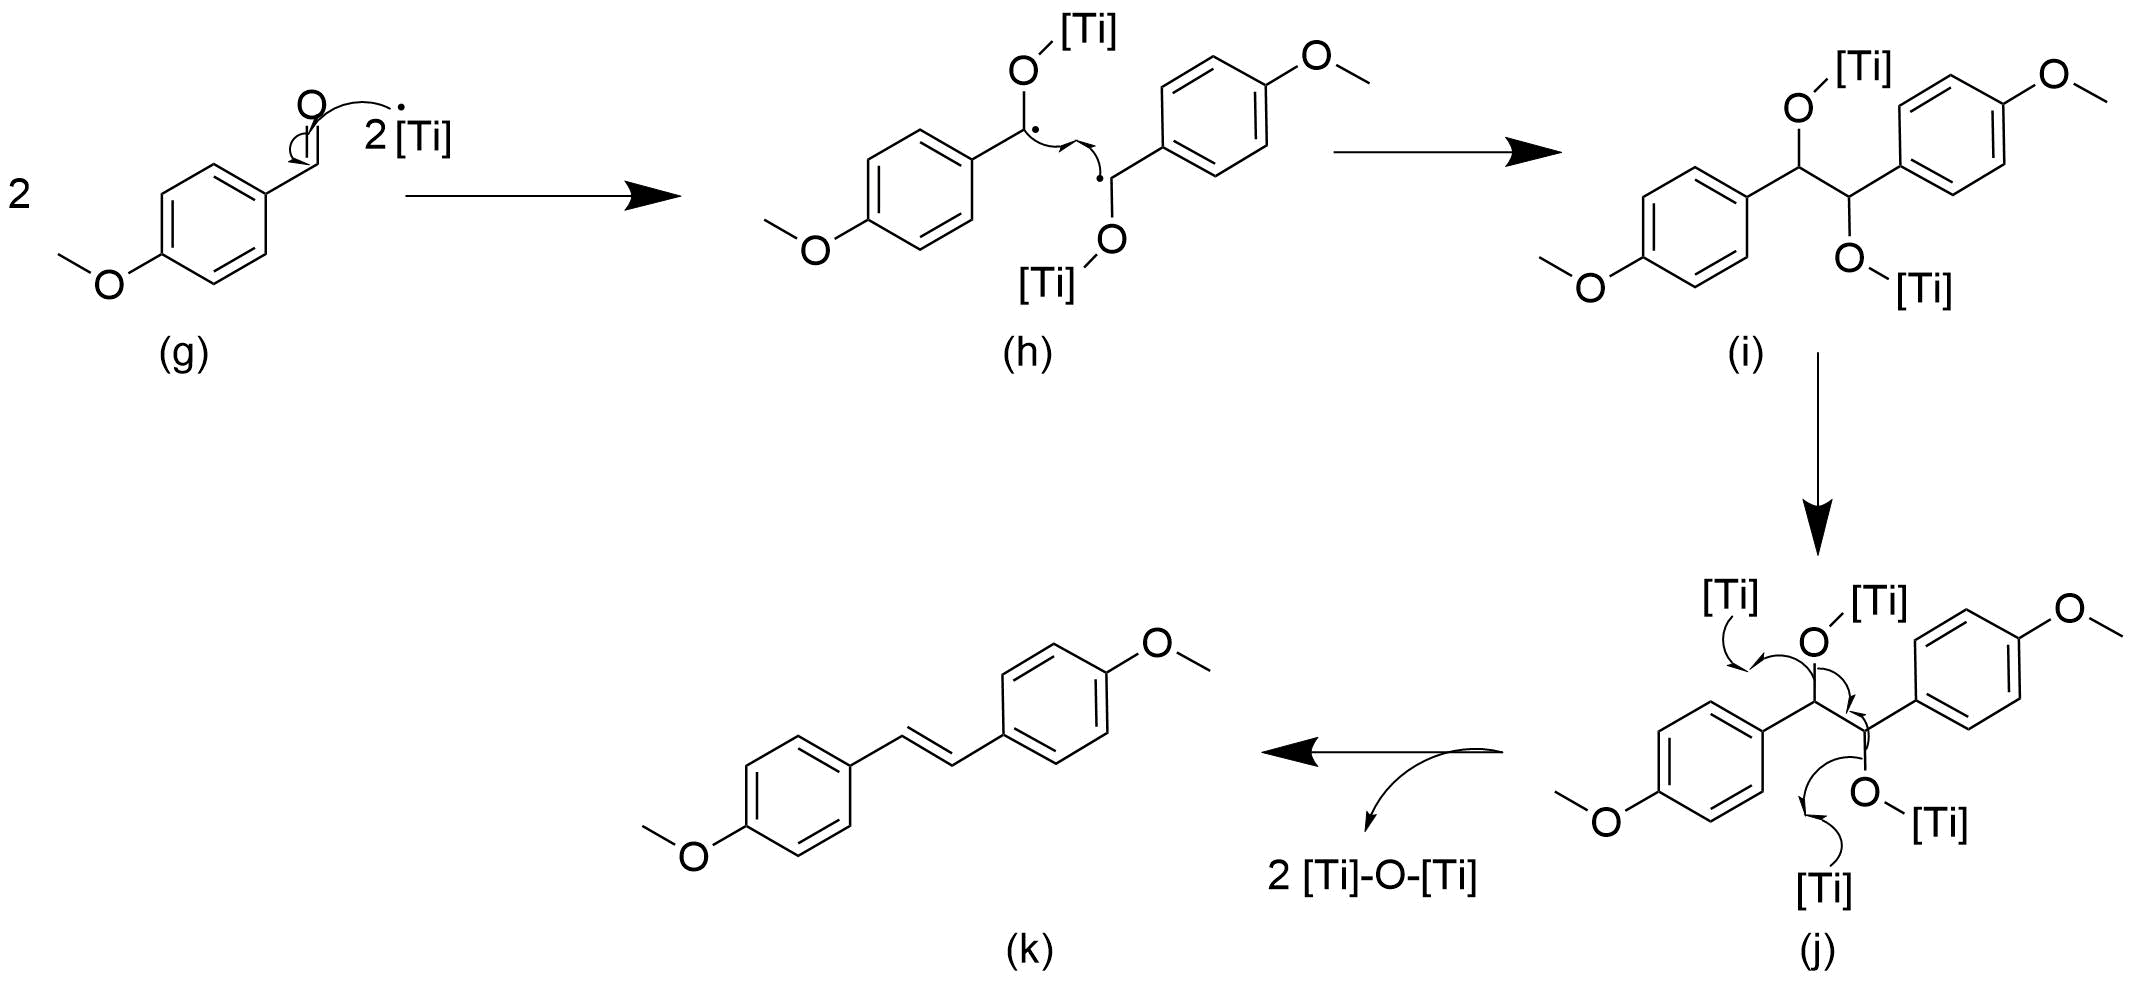
\includegraphics[width = \linewidth]{structures/mechanism2.png}
	\caption{Segundo mecanismo de reacci\'on propuesto \cite{Wang2010}.}
\end{scheme}

Es posible que ambos mecanismos ocurran en el medio de reacci\'on, de tal forma que se formen los subproductos \'oxido de titanio (IV), y \'oxido de titanio (III). Adem\'as ambos mecanismos son susceptibles a el efecto del agua en la reacci\'on, tanto los compuestos \textbf{(d)} como \textbf{(i)} en contacto con agua dar\'an lugar a la formaci\'on del diol, compuesto que se muestra en el \autoref{sch: diol}.
\begin{scheme}[h]
	\centering
	\scriptsize
	\begin{subfigure}[t]{0.49\linewidth}
		\centering
		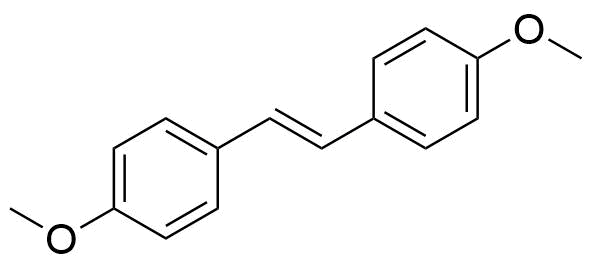
\includegraphics[width=0.9\linewidth]{structures/product.png}
		\caption{(\textit{E})-1,2-bis(4-metoxifenil)eteno}
		\label{sch: producto}
	\end{subfigure}
	\begin{subfigure}[t]{0.49\linewidth}
		\centering
		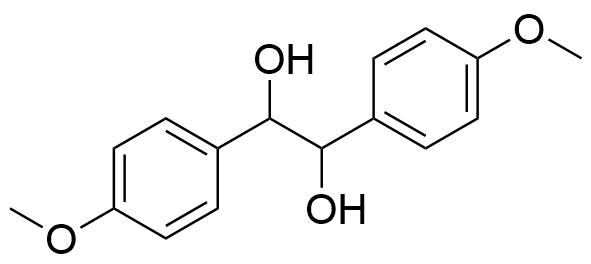
\includegraphics[width=0.9\linewidth]{structures/product2.png}
		\caption{(\textit{E})-1,2-bis(4-metoxifenil)etano-1,2-diol}
		\label{sch: diol}
	\end{subfigure}
	\caption{Productos de la reacci\'on.}
\end{scheme}

PRODUCTOS CRUZADOS CON ACIDO...

\section{Conclusiones}
\section{Secci\'on experimental}
50 mL de tetrahidrofurano previamente seco por 48 horas usando tamiz molecular, se agregan sobre un bal\'on de dos bocas junto con zinc (15.0 mmol) y cloruro de titanio (7.5 mmol). La soluci\'on se lleva a reflujo por 1 hora, pasada la cual se adiciona \textit{p}-metoxibenzaldehido (5.0 mmol). La reacci\'on se lleva a cabo a 55 $^\circ$C por 18 horas. La reacci\'on es tratada en 50 mL de \'acido clorh\'idrico 1 M. Se realiza una filtraci\'on en celita y una extracci\'on l\'iquido l\'iquido con dos lavados de 15 mL de diclorometano. El extracto se baña en salmuera y se extrae el sobrenadante, el cual se seca usando sulfato de magnesio y se evapora el disolvente.
%----------------------------------------------------------------------------------------
%	REFERENCE LIST
%----------------------------------------------------------------------------------------
\phantomsection
\bibliography{informe}
\bibliographystyle{achemso}
%----------------------------------------------------------------------------------------
\newpage
\onecolumn
\section{Informaci\'on suplementaria}\label{sec: complementaria}
\end{document}